Following the integration of updated high temperature opacities detiled in \S
\ref{sec:p1} we will investigate using the Jao-Gap color to age the local
solar neighboorhood.

Preilimiary modeling we have done, along with past literature [CITE]
demonstrates that the Jao Gap is expected to migrate along the main sequence as
a population of stars age. Stellar populations younger than $\sim 3 Gyr$ do not
show a gap. Once the gap forms it will migrate towrds brighter portions of the
CMD.

For this proposal we do not preform any rigorous statistical testing of whether
the differences in theoretical Jao Gap location could be discrimated between in
observational data; instead, choosing to save that element of the research for
thesis work proper. However, we do preform a qualitative test of the visual
distinguisability of the Jao Gap location for two sample sizes --- 500 and 1000
stars (Figure \ref{fig:JGTTE}).

\begin{equation}\label{eqn:IMF}
	\xi(m) = \xi_{0}\left(\frac{m}{M_{\odot}}\right)^{-2.68\pm0.09}
\end{equation}

We evolve models over an extremely finley sampled mass grid centered at the
theoretical Jao Gap location for a GS98 solar composition population of stars.
We then adopt the \citep{Sollima2019} IMF between 0.1 and 1 $M_{\odot}$
(Equation \ref{eqn:IMF}) to sample these evolved models. Model surface
gravities, effective temperatures, and luminosities are transformed into Gaia
magnitudes using bolometric correction tables provided by ESA\footnote{\url{https://gea.esac.esa.int/archive/documentation/GDR2/Data\_processing/chap\_cu5pho/sec\_cu5pho\_calibr/ssec\_cu5pho\_calibr\_extern.html}}. Uncertainty is injected by first transforming $G$, $BP$, and $RP$ flux
and flux uncertaninty measurments for all stars Gaia observed within 10pc to
magnitude and magnitude uncertaninties. Flux errors do not transform into
symetric magnitude errors; however, for small uncertaninties the transformation
may be approximated as symetric (Equations \ref{eqn:fluxerr2magerr} \&

\ref{eqn:sigfluxerr2magerr}).
\begin{equation}\label{eqn:fluxerr2magerr}
	M_{x} = -2.5\log_{10}(I_{x}) + ZP_{x}
\end{equation}
\begin{equation}\label{eqn:sigfluxerr2magerr}
	\sigma_{x} = \left(\frac{1.086\sigma_{I_{x}}}{I_{x}}\right)^{2} + ZP_{\sigma_{I_{x}}}^{2}
\end{equation}

Where $x$ is the band of interest, $I_{x}$ is the measured flux in that band,
and $ZP_{x}$ is the zero point offset in \texttt{VEGAMAG}. Following this
transformation, we fit a second-order polynominal to the magnitude error v.s.
magnitude for each band. This polynominal gives an approximation of the mean
uncertaninty for a given magnitude. For each point sampled from the IMF and set
of evolved models we add a sample from a normal distributions centered at 0 and
with a standard deviation equal to the evaluation of the optimized quadradic at
that points magnitude.

Figure \ref{fig:JGTTE} Panels A and B show (1 Gyr) do not show any visible Jao
Gap; whereas, Panels C, D, E, and F all do. Moreover, the location of the Gap
visible shiftes to lower magnitudes from 3 Gyr to 6 Gyrs. Note that this shift
is apparent in CMDs with both 1000s stars and those with 500 stars. In fact,
visually, this shift is clear with CMDs containing as few as 100 stars within
this mass range. Obviously, a simple visual identification is prone to
confirmation bias; however, we belive that these results are sufficent to
warrent a future, more rigorus, study.


\begin{figure}
	\centering
	\includegraphics[width=0.8\textwidth]{src/Figures/JaoGapTheoreticalTimeEvolution.pdf}
	\caption{Populations synthetis results for a mass range surrounding the
	theoretical location of the Jao Gap at 3 population ages and with different
	sample sizes. The superimposed color map is derived from a gaussian
	kernel-density-estimation run on the displayed points. This is included to
	better illustrate the gap location.}
	\label{fig:JGTTE}
\end{figure}


Models predict that the location of the Jap Gap will shift with population age
[CITATION]; in fact, we see this behavior, gap colors reddening as populations
age, in populations evolved with DSEP [FIGURE] which span the mass range of the
gap.

[DETAILS ON KINEMATIC AGEING]

We propose to model a population of stars of various ages and mettalicities
sampled from the local stellar neighboorhood. Each of these stars will be
assigned kinematics --- again sampled from empirical distributions. We will
then extract kinematically derived ages from this population and use these to
segregate stars into rough age bins. Finally, we will measure if difference in
Jao gap locations are statistically distinquishable between these rough age bins.

\begin{figure}
	\centering
	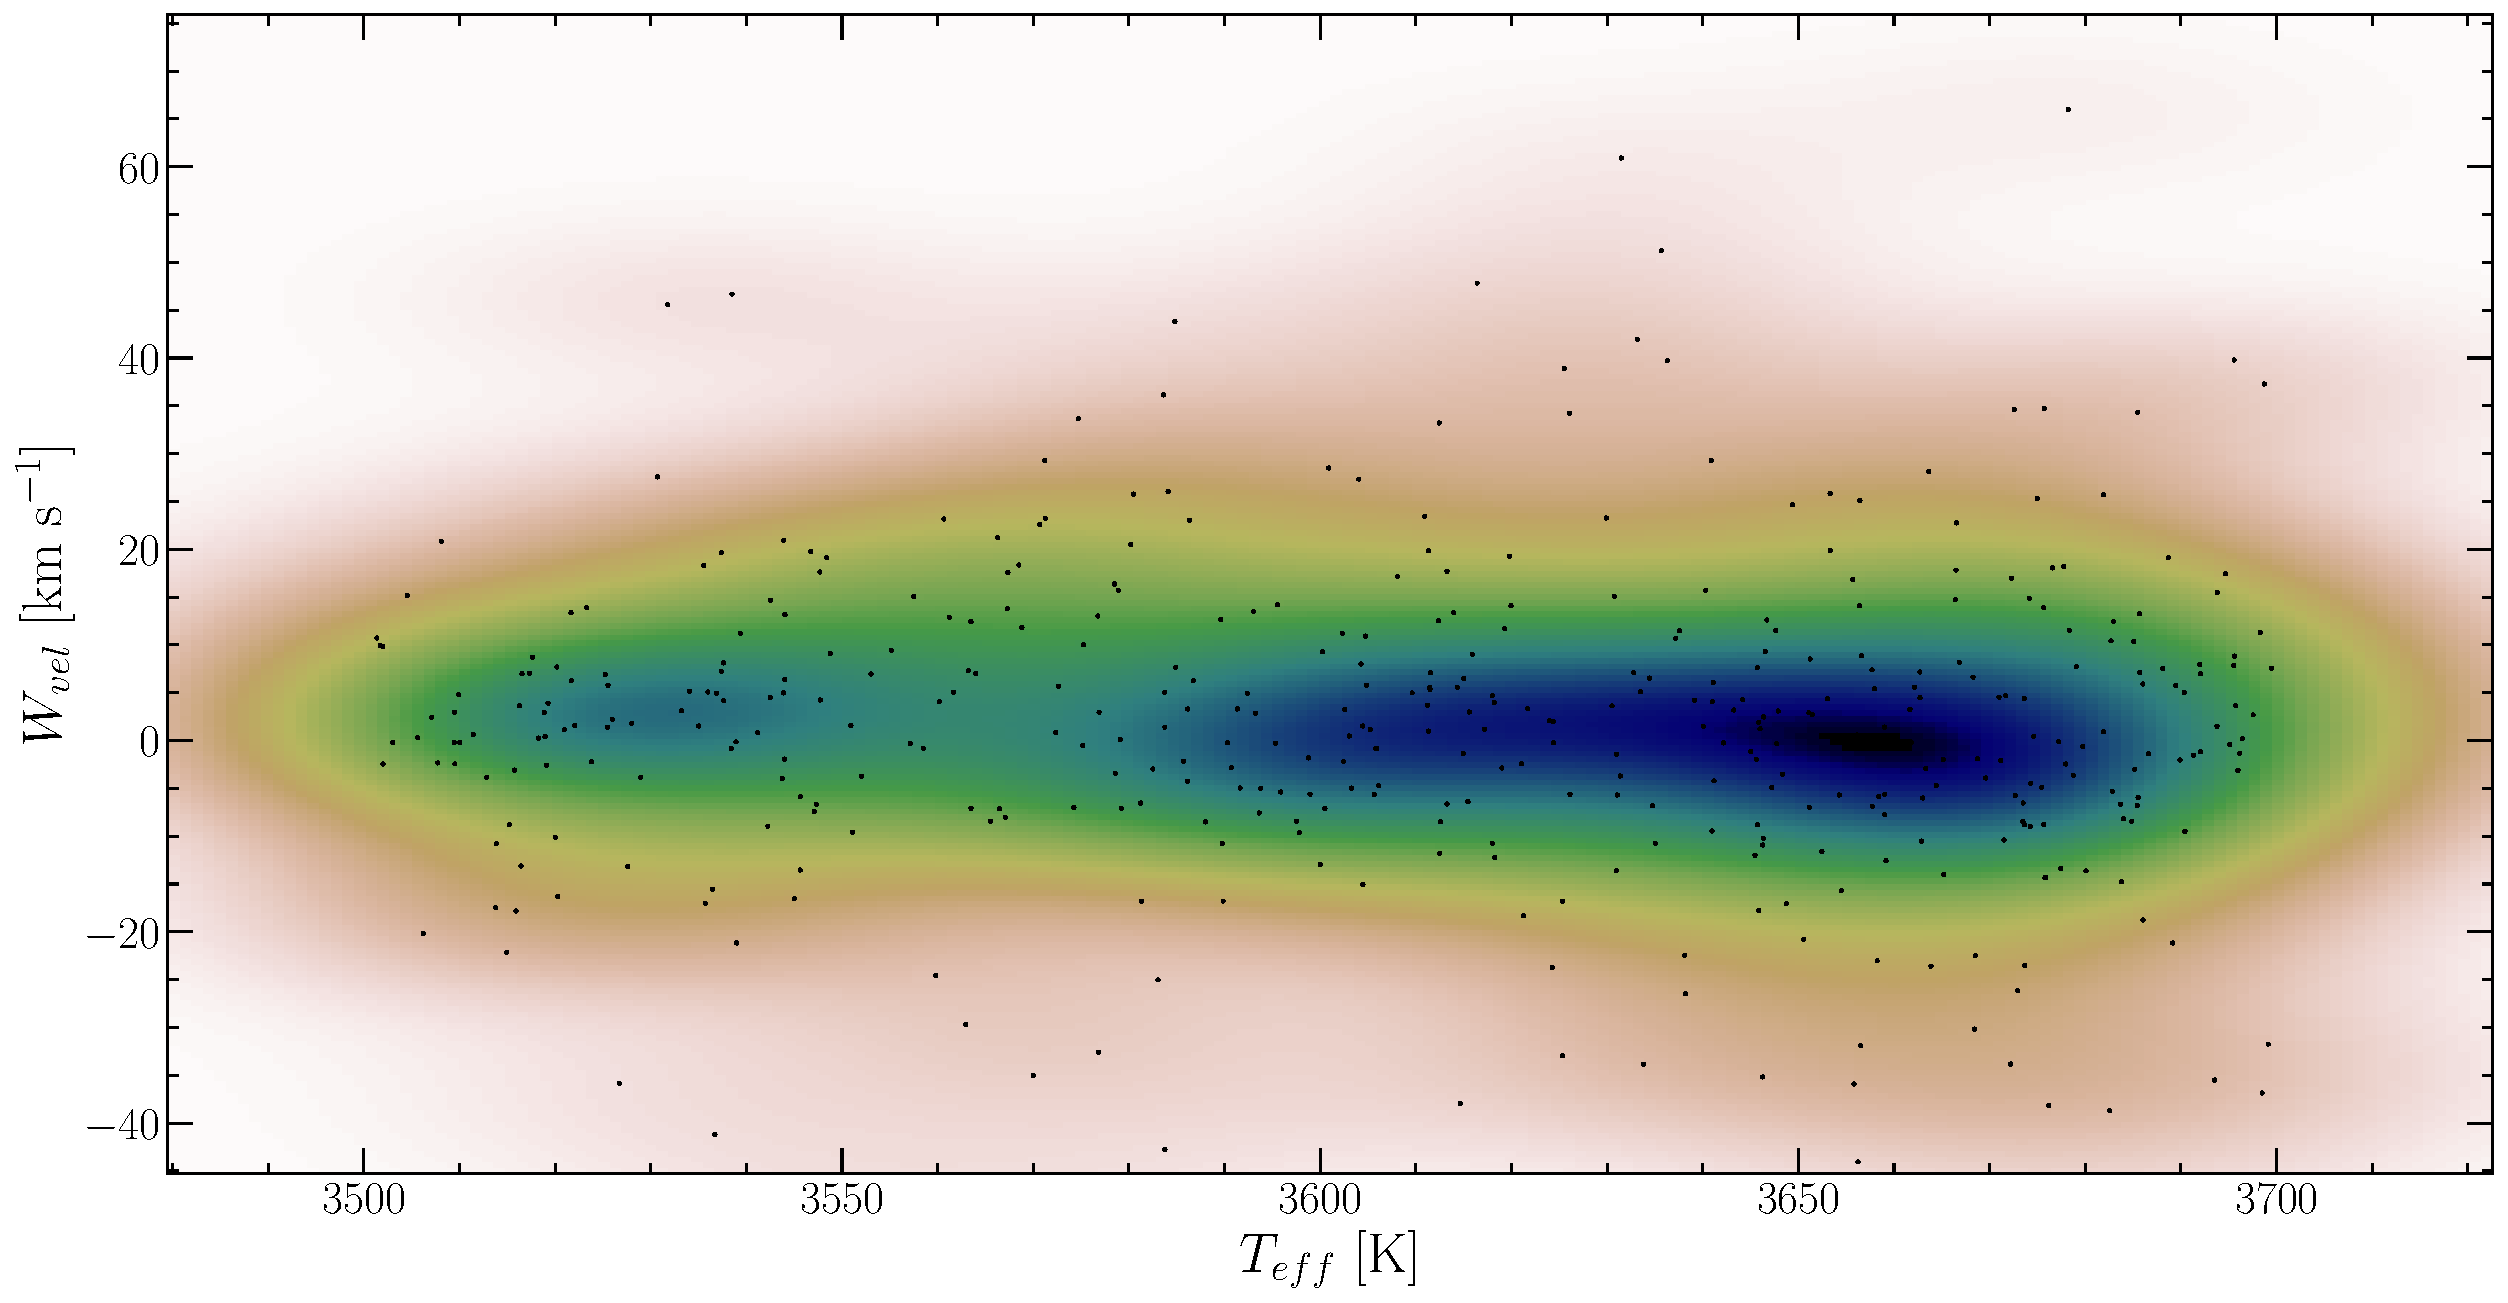
\includegraphics[width=0.75\textwidth]{src/Figures/LuEtAlKDE.pdf}
	\caption{Kernel Density Estimation function of the gyro-kinematically
	infered velocity vs. effetive temperature. This sample is selected from
	\citet{Lu2021} and cut between $T_{eff} < 3800$ K and $T_{eff} > 3500$ K.}
	\label{fig:LuKde}
\end{figure}
